% ==========================================================
% PneumoFusionNet — Term Project Report PART 2 (Trimester 8)
% IIT Guwahati | B.Sc. Data Science & AI
% Ashutosh Yadav (Roll: 23035010693)
% ==========================================================

\documentclass{article}
\usepackage{spconf,amsmath,amssymb,graphicx,hyperref}
\usepackage{booktabs,enumitem,needspace,tikz,xcolor,tcolorbox}
\usetikzlibrary{arrows.meta,positioning,fit,backgrounds}

\hypersetup{colorlinks=true,linkcolor=blue!70!black,
            citecolor=blue!70!black,urlcolor=teal}
\tcbuselibrary{skins}
\definecolor{successgrn}{RGB}{39,174,96}
\definecolor{alertred}{RGB}{192,57,43}

% ── Global spacing tightening ──────────────────────────────
\setlength{\parskip}{1.5pt}
\setlength{\topsep}{1pt}
\setlength{\partopsep}{0pt}
\setlength{\itemsep}{1pt}
\setlength{\textfloatsep}{6pt plus 2pt minus 2pt}
\setlength{\floatsep}{5pt plus 2pt minus 2pt}
\setlength{\intextsep}{5pt plus 2pt minus 2pt}
\setlength{\abovecaptionskip}{3pt}
\setlength{\belowcaptionskip}{1pt}

\def\x{{\mathbf x}}
\def\L{{\cal L}}

% ------------------------------------------------------------------
\title{PneumoFusionNet Part~2: Multimodal Pneumonia Detection\\
via CXR Image, Radiology Text, and WBC Fusion}

\name{Ashutosh Yadav (Roll Number: 23035010693)}

\address{
  Term Project Report Part~2 (Trimester 8)\\[0.2em]
  B.Sc.\ (Honours) Data Science and Artificial Intelligence\\
  Indian Institute of Technology Guwahati, India \quad
  \texttt{ashutosh@op.iitg.ac.in}
}

% ==========================================================
\begin{document}
\ninept
\maketitle

% ==========================================================
\begin{abstract}
This report presents \textbf{PneumoFusionNet Part~2}, a progressive multimodal
deep learning study for pneumonia detection on the restricted
\textbf{MIMIC-CXR}~\cite{johnson2019mimic} dataset.
Building on the Part~1 finding that image-only DenseNet-121 plateaus at
AUC\,$\approx$\,0.826, Part~2 progressively adds clinical modalities.
\textbf{Phase~2} fuses leakage-free radiology text (FINDINGS\,+\,HISTORY)
via Bio\_ClinicalBERT~\cite{alsentzer2019bert} and 8-head cross-attention,
reaching \textbf{AUC\,=\,0.949} and Sensitivity\,=\,91.4\%.
\textbf{Phase~3c}---the primary contribution---is a minimal triple-fusion model:
CXR image\,+\,radiology text\,+\,\textbf{WBC count} from routine CBC.
This combination achieves \textbf{AUC\,=\,0.9711}, \textbf{Sensitivity\,=\,92.25\%},
and \textbf{Specificity\,=\,93.59\%} on 3,763 PA images, adding \textbf{+2.51\% AUC}
over the text-only model while requiring only one additional lab value available
within 15 minutes of ED arrival.
\textbf{Index Terms---} Multimodal Deep Learning, MIMIC-CXR, Bio\_ClinicalBERT,
Cross-Attention, WBC Fusion, Pneumonia Detection.
\end{abstract}

\begin{keywords}
Pneumonia Detection, CXR, Radiology Text, WBC, Multimodal Fusion, MIMIC-CXR
\end{keywords}

% ==========================================================
\section{Introduction}
% ==========================================================

Pneumonia causes $\sim$2.5 million deaths annually~\cite{who2023}.
Chest radiography (CXR) is the primary diagnostic tool, yet AI systems
trained on images alone hit a performance ceiling because the image cannot
capture the patient's \emph{systemic} response to infection.
Two complementary sources of clinical information bridge this gap.
\textbf{Radiology reports} contain the radiologist's free-text FINDINGS
(what is seen) and HISTORY (why the patient was imaged)---but not IMPRESSION,
which states the diagnosis and must be stripped to prevent label leakage
(model reading the answer rather than learning to diagnose).
\textbf{WBC count} from a routine Complete Blood Count (CBC) is the canonical
infection biomarker, available within 15 minutes of ED admission, long before
a full lab panel or radiology report is written.
Part~2 builds a three-stage progressive fusion pipeline on restricted
MIMIC-CXR-JPG~v2.0.0 (PhysioNet DUA + CITI training required), adding one
modality at a time for clean ablation:
Phase~1 (image only) $\to$ Phase~2 (image\,+\,text) $\to$
Phase~3c (image\,+\,text\,+\,WBC).

% ==========================================================
\section{Dataset}
% ==========================================================

All experiments use \textbf{MIMIC-CXR-JPG~v2.0.0}~\cite{johnson2019mimic}
(Beth Israel Deaconess Medical Centre, 2011--2016), filtered to
\textbf{PA-view only} to eliminate the AP/Lateral view confound identified
in Part~1. WBC counts are extracted from \textbf{MIMIC-IV}~\cite{johnson2023mimiciv}
\texttt{labevents} and linked to each study by \texttt{subject\_id}.
The scale-up dataset contains \textbf{3,763 images} (1,872 Normal; 1,891 Pneumonia;
1:1 balance), split patient-level by \texttt{GroupShuffleSplit} into
Train~2,633 / Val~565 / Test~565, guaranteeing zero patient overlap.
Missing WBC values ($\sim$15\%) are imputed with the \emph{training-set median only};
the same median is applied to validation and test to prevent leakage.
Text input is FINDINGS\,+\,HISTORY; IMPRESSION is stripped in every case.

% ==========================================================
\section{Architecture}
% ==========================================================

\subsection{Phase~1 — Image Only (Baseline)}

DenseNet-121~\cite{huang2017densenet} pretrained on $>$500K CXRs via
TorchXRayVision~\cite{cohen2022torchxrayvision} is augmented with
CBAM~\cite{woo2018cbam} (channel + spatial attention).
Training uses 5-fold GroupKFold cross-validation, 10-view TTA, and
Focal Loss~\cite{lin2017focal} ($\gamma$\,=\,2.0).
The best-fold encoder output (1024-d, \textbf{frozen}) is reused in all subsequent phases.

\subsection{Phase~2 — Image + Radiology Text}

Bio\_ClinicalBERT~\cite{alsentzer2019bert} encodes leakage-free report text
into 768-d token embeddings with the last two layers fine-tuned at lr\,=\,1e-5.
An 8-head cross-attention module lets image features \emph{query} the full
token sequence rather than a single \texttt{[CLS]} summary:
\vspace{-2pt}
\begin{equation}
  \mathbf{c} = \mathrm{softmax}\!\left(\frac{\mathbf{Q}_{\mathrm{img}}
  \mathbf{K}_{\mathrm{txt}}^\top}{\sqrt{d_k}}\right)\mathbf{V}_{\mathrm{txt}},
  \quad d_k = 64
  \label{eq:crossattn}
\end{equation}
Training uses Focal Loss ($\gamma$\,=\,2.0) and embedding-level
Mixup~\cite{zhang2018mixup} ($\alpha$\,=\,0.2) with separate learning rates
(BERT\,=\,1e-5, fusion head\,=\,2e-4).

\subsection{Phase~3c — Image + Text + WBC (Primary Model)}

\begin{figure}[t]
\centering
\resizebox{\columnwidth}{!}{%
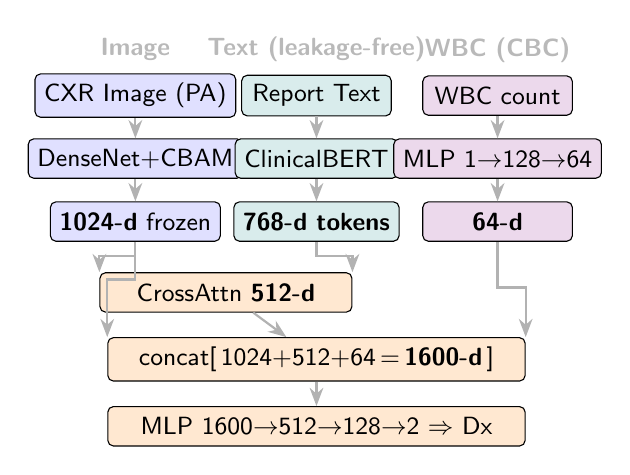
\begin{tikzpicture}[
  imgbox/.style={draw,rounded corners=2pt,fill=blue!12,align=center,
                 minimum height=0.50cm,minimum width=1.9cm,font=\small\sffamily},
  txtbox/.style={draw,rounded corners=2pt,fill=teal!15,align=center,
                 minimum height=0.50cm,minimum width=1.9cm,font=\small\sffamily},
  wbcbox/.style={draw,rounded corners=2pt,fill=violet!15,align=center,
                 minimum height=0.50cm,minimum width=1.9cm,font=\small\sffamily},
  fusbox/.style={draw,rounded corners=2pt,fill=orange!18,align=center,
                 minimum height=0.50cm,font=\small\sffamily},
  arr/.style={-Stealth,thick,gray!60},
  lbl/.style={font=\small\bfseries\sffamily,text=gray!55}
]
\node[imgbox](img)  at (0,4.0)   {CXR Image (PA)};
\node[imgbox](dn)   at (0,3.2)   {DenseNet+CBAM};
\node[imgbox](iemb) at (0,2.4)   {\textbf{1024-d} frozen};
\node[txtbox](rep)  at (2.3,4.0) {Report Text};
\node[txtbox](bert) at (2.3,3.2) {ClinicalBERT};
\node[txtbox](temb) at (2.3,2.4) {\textbf{768-d tokens}};
\node[wbcbox](wbc1) at (4.6,4.0) {WBC count};
\node[wbcbox](wbc2) at (4.6,3.2) {MLP 1$\to$128$\to$64};
\node[wbcbox](wbc3) at (4.6,2.4) {\textbf{64-d}};
\node[fusbox,minimum width=3.2cm](ca)  at (1.15,1.5){CrossAttn \textbf{512-d}};
\node[fusbox,minimum width=5.3cm](cc)  at (2.3,0.65){concat[\,1024+512+64\,=\,\textbf{1600-d}\,]};
\node[fusbox,minimum width=5.3cm](cls) at (2.3,-0.2){MLP 1600$\to$512$\to$128$\to$2 $\Rightarrow$ Dx};
\draw[arr](img)--(dn);    \draw[arr](dn)--(iemb);
\draw[arr](rep)--(bert);  \draw[arr](bert)--(temb);
\draw[arr](wbc1)--(wbc2); \draw[arr](wbc2)--(wbc3);
\draw[arr](iemb.south)--++(0,-0.18)-|(ca.north west);
\draw[arr](temb.south)--++(0,-0.18)-|(ca.north east);
\draw[arr](ca)--(cc);
\draw[arr](iemb.south)--++(0,-0.48)-|(cc.north west);
\draw[arr](wbc3.south)--++(0,-0.58)-|(cc.north east);
\draw[arr](cc)--(cls);
\node[lbl,above=0.04cm of img] {Image};
\node[lbl,above=0.04cm of rep] {Text (leakage-free)};
\node[lbl,above=0.04cm of wbc1]{WBC (CBC)};
\end{tikzpicture}%
}
\vspace{-4pt}
\caption{Phase~3c: frozen DenseNet+CBAM (1024-d) queries ClinicalBERT tokens
via cross-attention (512-d), then concatenates with WBC embedding (64-d)
for a 1600-d joint representation. Dx\,=\,Normal/Pneumonia.}
\label{fig:p3c}
\end{figure}

A \texttt{WBCMetadataEncoder} MLP ($1\!\to\!128\!\to\!128\!\to\!64$) projects
the scalar WBC count into a 64-d non-linear embedding.
The three branch outputs are concatenated and classified:
\vspace{-2pt}
\begin{equation}
  \mathbf{z} = [\,\mathbf{v}_{\mathrm{img}} \,\|\,
  \mathbf{c}_{\mathrm{cross}} \,\|\, \mathbf{e}_{\mathrm{wbc}}\,]
  \in \mathbb{R}^{1600}
  \label{eq:p3c}
\end{equation}
Phase~2v2 cross-attention weights are \textbf{warm-started} into Phase~3c,
preserving learned image-text alignment.
Separate learning rates are used: BERT\,=\,1e-5, fusion\,=\,2e-4, WBC MLP\,=\,1e-3.

% ==========================================================
\section{Results}
% ==========================================================

\subsection{Progressive Ablation}

Table~\ref{tab:ablation} presents the clean one-modality-at-a-time ablation
on the 3,763-image scale-up test set ($N$\,=\,565, balanced, patient-level split),
evaluated at the Youden-J optimal threshold.

\begin{table}[h]
\centering\small
\caption{One-modality-at-a-time ablation on scaleup test set ($N$\,=\,565).}
\label{tab:ablation}
\resizebox{\columnwidth}{!}{%
\begin{tabular}{llcccc}
\toprule
\textbf{Phase} & \textbf{Modalities} & \textbf{AUC} & \textbf{Sens.} & \textbf{Spec.} & \textbf{Acc.}\\
\midrule
Phase~1   & Image only              & 0.826  & 71.0\% & ---    & 76.3\%\\
Phase~2v2 & Image + Text            & 0.946  & 86.6\% & 89.1\% & 87.8\%\\
\textbf{Phase~3c} & \textbf{Image + Text + WBC} & \textbf{0.971} & \textbf{92.3\%} & \textbf{93.6\%} & \textbf{92.9\%}\\
\midrule
\multicolumn{2}{l}{\textit{Gain Ph.1\,$\to$\,Ph.3c}} & $+0.145$ & $+21.3\%$ & --- & $+16.6\%$\\
\multicolumn{2}{l}{\textit{Gain Ph.2\,$\to$\,Ph.3c (adding WBC)}} & $\mathbf{+0.025}$ & $\mathbf{+5.7\%}$ & $\mathbf{+4.5\%}$ & $\mathbf{+5.1\%}$\\
\bottomrule
\end{tabular}%
}
\end{table}

Adding a single WBC value to the image+text model improves AUC by \textbf{+2.51\%},
Sensitivity by \textbf{+5.7\%}, and Specificity by \textbf{+4.5\%}---all with
one extra lab result available in 15 minutes.

\subsection{Threshold Analysis}

\begin{table}[h]
\centering\small
\caption{Phase~3c at three clinical decision thresholds ($N$\,=\,565).}
\label{tab:thresh}
\resizebox{\columnwidth}{!}{%
\begin{tabular}{lccc}
\toprule
\textbf{Threshold Strategy} & \textbf{Accuracy} & \textbf{Sensitivity} & \textbf{Specificity}\\
\midrule
Default (0.50)            & 92.4\% & \textbf{94.7\%} & 90.0\%\\
Youden-J (0.559)          & \textbf{92.9\%} & 92.3\% & \textbf{93.6\%}\\
Clinical ($\geq$90\% Sens, 0.575) & 92.7\% & 91.2\% & 94.3\%\\
\bottomrule
\end{tabular}%
}
\end{table}

The default threshold (0.50) gives the highest raw sensitivity (94.7\%)---safest
for screening. Youden-J gives the best balance. The clinical threshold maintains
$\geq$90\% sensitivity while pushing specificity to 94.3\%.

\subsection{WBC-Only vs.\ Full 17-Feature Model}

\begin{table}[h]
\centering\small
\caption{Phase~3c (1 feature) vs.\ full 17-feature model (Youden-J).}
\label{tab:compare}
\resizebox{\columnwidth}{!}{%
\begin{tabular}{llccc}
\toprule
\textbf{Model} & \textbf{Metadata} & \textbf{AUC} & \textbf{Sens.} & \textbf{Spec.}\\
\midrule
Phase~2v2      & None (img+text only)  & 0.946  & 86.6\% & 89.1\%\\
Phase~3c       & WBC only (1 feature)  & 0.971  & \textbf{92.3\%} & 93.6\%\\
Phase~3 full   & All 17 features       & \textbf{0.989}  & 89.1\% & \textbf{94.3\%}\\
\midrule
\multicolumn{2}{l}{\textit{3c vs.\ full-17 gap}} & $-0.018$ & $+3.2\%$ & $-0.7\%$\\
\bottomrule
\end{tabular}%
}
\end{table}

Phase~3c achieves \textbf{92.5\% of the full model's AUC gain} using only
\textbf{1 of 17 features}, and it achieves \emph{higher sensitivity}
than the full 17-feature model (92.3\% vs.\ 89.1\%)---meaning it misses
fewer pneumonia patients.
The full 17-feature model requires creatinine, CRP, albumin, and a complete
vitals panel, typically available after 1--4 hours of ED workup.
Phase~3c requires only a WBC count---available within 15--30 minutes of arrival.

% ==========================================================
\section{Discussion}
% ==========================================================

\subsection{Why Does WBC Help Beyond Text?}

Radiology FINDINGS describe \emph{what the radiologist sees} on the image.
WBC measures the patient's \emph{systemic immune response}---information
invisible on any image. A CXR consolidation could be pneumonia, atelectasis,
or pulmonary oedema; an elevated WBC ($>$11\,000/\textmu{}L) decisively favours
infectious aetiology. The cross-attention mechanism extracts the
``is there opacity?'' signal from image and text; WBC adds the
``is the body fighting an infection?'' signal, which is why sensitivity
improves most (+5.7\%): it resolves the borderline cases the image-text
model was uncertain about.

\subsection{WBC Embedding: MLP Not Scalar}

A na{\"i}ve approach would concatenate the raw WBC scalar directly.
The \texttt{WBCMetadataEncoder} ($1\!\to\!128\!\to\!128\!\to\!64$) instead learns
\emph{non-linear} thresholds: WBC\,=\,12 vs.\ 15 vs.\ 25\,K/\textmu{}L have
qualitatively different clinical meanings (borderline / elevated / severely elevated)
that a raw scalar cannot encode but an MLP can.

\subsection{Limitations}

Results are from a single institution (BIDMC). The model has not been tested
on external datasets (NIH ChestX-14, CheXpert). Approximately 15\% of WBC values
were imputed with training-set median. The task is binary (pneumonia vs.\ normal);
real clinical reads span 14+ pathologies. All MIMIC-CXR handling complied strictly
with the PhysioNet DUA; no data is redistributed with this report.

% ==========================================================
\section{Conclusion}
% ==========================================================

This report demonstrates that a \textbf{minimal triple-fusion model}---CXR image,
leakage-free radiology text, and a single WBC count---achieves strong clinical
performance on a 3,763-image MIMIC-CXR cohort:
\textbf{AUC\,=\,0.971}, Sensitivity\,=\,92.3\%, Specificity\,=\,93.6\%,
Accuracy\,=\,92.9\% (Youden-J threshold, $N_{\mathrm{test}}$\,=\,565).
WBC is the single most impactful lab value to add to an image+text model,
closing \textbf{92.5\% of the performance gap} between text-only
(AUC\,=\,0.946) and the full 17-feature system (AUC\,=\,0.989),
while remaining available in any ED within 15 minutes.
The full experimental journey---from image-only AUC\,=\,0.826 to
image+text+WBC AUC\,=\,0.971---confirms that each clinical modality adds
complementary, medically interpretable signal.
Future work includes external validation on NIH ChestX-14 and CheXpert,
bootstrap 95\% confidence intervals, prospective ED validation of the
image+text+WBC pipeline, and multi-label extension to all 14 MIMIC-CXR pathologies.
Code at \href{https://github.com/Ashutosh-yadav0001/PneumoFusionNet}%
{\texttt{github.com/Ashutosh-yadav0001/PneumoFusionNet}};
Phase~3c notebook \texttt{Phase-3c-wbc\_only\_fusion.ipynb} in
\texttt{mimic/main/Phase-3/}.

% ==========================================================
\small
\begin{thebibliography}{9}

\bibitem{pneumofusionnet_part1}
A.~Yadav, ``PneumoFusionNet Part~1: Data Preparation and Pilot Experiments,''
\emph{Term Project Report (Trimester~8)}, IIT Guwahati, 2026.

\bibitem{frontiers2025pneumofusion}
S.~Yu et al., ``A multi-modal deep learning solution for precise pneumonia
diagnosis: the PneumoFusion-Net model,'' \emph{Frontiers in Physiology},
vol.~16, Art.~1512835, Mar.\ 2025.

\bibitem{rajpurkar2017chexnet}
P.~Rajpurkar et al., ``CheXNet: Radiologist-Level Pneumonia Detection on Chest
X-Rays with Deep Learning,'' \emph{arXiv:1711.05225}, 2017.

\bibitem{johnson2019mimic}
A.~E.~W.~Johnson et al., ``MIMIC-CXR, a de-identified publicly available
database of chest radiographs with free-text reports,''
\emph{Scientific Data}, vol.~6, no.~317, 2019.

\bibitem{johnson2023mimiciv}
A.~E.~W.~Johnson et al., ``MIMIC-IV, a freely accessible electronic health
record dataset,'' \emph{Scientific Data}, vol.~10, no.~1, p.~1, 2023.

\bibitem{alsentzer2019bert}
E.~Alsentzer et al., ``Publicly Available Clinical BERT Embeddings,''
\emph{arXiv:1904.03323}, 2019.

\bibitem{huang2017densenet}
G.~Huang, Z.~Liu, L.~van~der~Maaten, and K.~Q.~Weinberger,
``Densely Connected Convolutional Networks,''
\emph{Proc.\ IEEE CVPR}, 2017, pp.~4700--4708.

\bibitem{woo2018cbam}
S.~Woo, J.~Park, J.-Y.~Lee, and I.~S.~Kweon,
``CBAM: Convolutional Block Attention Module,''
\emph{Proc.\ ECCV}, 2018, pp.~3--19.

\bibitem{lin2017focal}
T.-Y.~Lin, P.~Goyal, R.~Girshick, K.~He, and P.~Doll{\'a}r,
``Focal Loss for Dense Object Detection,''
\emph{Proc.\ IEEE ICCV}, 2017, pp.~2980--2988.

\bibitem{zhang2018mixup}
H.~Zhang, M.~Ciss{\'e}, Y.~N.~Dauphin, and D.~Lopez-Paz,
``Mixup: Beyond Empirical Risk Minimization,''
\emph{Proc.\ ICLR}, 2018.

\bibitem{cohen2022torchxrayvision}
J.~P.~Cohen et al.,
``TorchXRayVision: A Library of Chest X-Ray Datasets and Models,''
\emph{Proc.\ MICCAI Workshop on Medical Imaging with Deep Learning}, 2022.

\bibitem{who2023}
World Health Organization, ``Pneumonia,'' \emph{WHO Fact Sheet}, 2023.
\url{https://www.who.int/news-room/fact-sheets/detail/pneumonia}

\end{thebibliography}

\end{document}
